\documentclass{standalone}
% preamble: usepackage, etc.
\begin{document}

\thesischapterexordium

\section{研究工作的背景与意义}
随着城市交通网络的发展和交通工具的进步,针对路径规划问题设计的各种系统和算法逐渐在现实生活中被广泛的应用,比如在日常驾驶出行或乘坐公共交通等情景中,人们越来越频繁的使用这一功能。同时随着交通网络复杂度提高,规模增大,多种交通工具的出现以及城市堵车给城市交通网络带来的随机性和动态性,这给传统的路径规划问题带来了全面的挑战。同样,随着自动驾驶技术的发展,路径规划问题作为自动驾驶的导航模块中重要的部分同样扮演者不可或缺的角色。因此如何更好的设计出更强大,更具灵活性的,更高效的路径规划算法具有重要的发展意义,而这也成为了当前各国学者的研究热点之一。

% \footnote{脚注序号“\ding{172},……,\ding{180}”的字体是“正文”,不是“上标”,序号与脚注内容文字之间空1个半角字符,脚注的段落格式为:单倍行距,段前空0磅,段后空0磅,悬挂缩进1.5字符;中文用宋体,字号为小五号,英文和数字用Times New Roman字体,字号为9磅;中英文混排时,所有标点符号(例如逗号“,”、括号“()”等)一律使用中文输入状态下的标点符号,但小数点采用英文状态下的样式“.”。}

\section{路径规划问题的国内外研究历史与现状}
路径规划问题,简单而言是在某一个环境中,给定起点和终点,输出一条最优路径的问题。根据问题建模形式不同,分为两类解决方法,第一类为基于图的搜索算法,第二类为为基于采样的规划方法。基于采样的方法是为了解决三维空间或较高复杂度情况下的机器人路径规划问题,一般并不通过构建基于拓扑结构的图进行处理,而是采用在地图上随机撒一定密度的粒子来抽象实际的地图进行辅助规划。这类规划问题包括了 PRM\citing{PRM}, RRT\citing{RRT}等一系列方法。
在本文中,我们重点讨论基于图的路径规划发算法,基于图的形式意味着我们拥有交通网络环境的全局信息,着包括了图中边的集合,点的集合以及边上的权值信息等。基于完备地图的路径规划最早被转换为图论中的最短路径问题,最短路径问题根据图的类型和需求的不同,首先分为无向图上的最短路径、有向图上的最短路径、单源最短路,多源最短路等等。根据图性质的不同,分为静态图上的最短路、动态图上的最短路、具有时序依赖的最短路、参数化的最短路、可替换性的最短路、可替代性最短路、随机性图上的最短路以及带权重的近似最短路等问题。\par

Edsger W. Dijkstra 最早于1956年,提出了著名的 $Dijkstra$\citing{Dijkstra} 算法,给出了基于静态图的单源最短路算法,随后包括 Bellman-Ford, $A^*$ search, Floyd-Warshall Johnson's algorithm, Viterbi algorithm等被相继提出,在一定程度上都降低了最短路算法的时空复杂度。随着研究的深入,当前最短路径算法已经组成了一个庞大的算法群,国外的学者根据问题形式和算法形式的不同,做了如图\ref{1-1}所示的总结和分类\citing{suveryOnShortestPath}。首先基于静态图(Static)的问题中,图的结构,包括点集合、边集以及权重保持不变,相应的算法分为单源最短路(Single Source),多源最短路(All Paris)等。基于预处理加速的方法(Distance Oracle),基于目标导向(Goal Directed)的优化方法,分层(Hierarchical)的方法等。基于动态图(Dynamic)的问题中,图的结构可能会发生变化,例如插入、删除边或者点,更新边上的权值等操作。 相应的算法分为单源最短路和多源最短路的算法。时序依赖(Time-dependent)的最短路问题中,图的动态性一般依赖于时序变化,而相应的算法也融合了多种预测算法对图的时序特性进行越策。参数化(Parametric)的最短路径问题中,算法基于某些具体参数的值计算最短路径。可替换性(Replacement)最短路问题中,算法需给出不包含任意某一条边的最短路的解的集合,而这类算法往往会重复使用先前的计算结果。可替代性(Alternative)最短路问题中,算法要求给出一条不包含某一特定边的最短路径。带权重(Weight-Regions)的近似最短路问题为找到在某一类权重下最优的近似最短路径。带有随机性(Stochastic)的图的最短路问题为通过将边的权重建模为随机变量,然后进行求解。\par
\begin{figure}[H]
	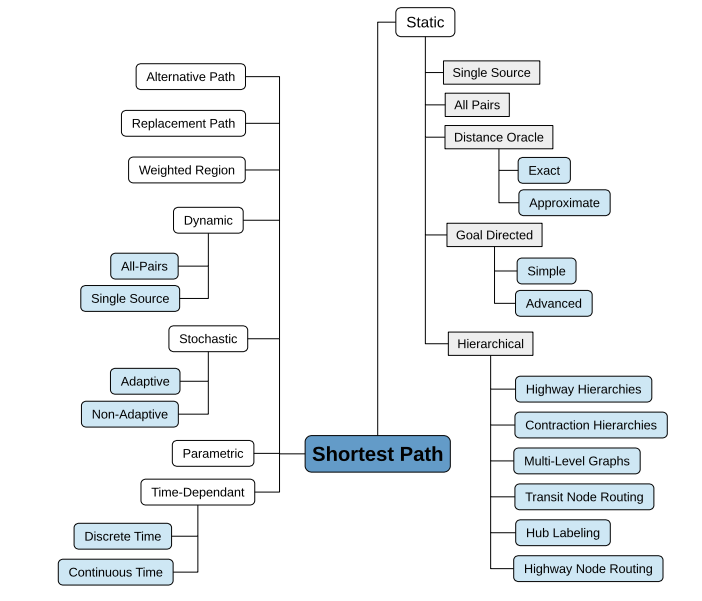
\includegraphics[width=12.0cm]{1-1.png}
	\caption{最短路径算法分类图}
	\label{1-1}
\end{figure}

但随着交通环境复杂度的增加(大陆级别的地图范围)和用户需求的增加(例如需要考虑多种交通工具的组合,倾向选择公共交通方式,选择非收费路段,电动车行驶路径限制和充电问题等)。现有的各种算法已经不能很好的解决路径规划问题。因此各国学者和研究机构,针对不同的场景,提出了相应改进的算法。\par

在动态图最短路径问题中,Demetrescu 和 Italiano 提出了在有向图上的多源最短算法\citing{Demetrescu},每条边可以存储某一固定数量的权值,算法的复杂度为 $O(Sn^{2.5}log^3n)$,Bernsteini 提出了一个 $(2+\epsilon)$算法\citing{Bernstein},解决了有向图上的多源最短路问题,其更新的时间复杂度接近线性,查询时间为$O(loglogn)$。Henzinger 等人\citing{Henzinger2013Dynamic}通过改进 Shiloach 和 Even 提出的fast deterministic 算法\citing{fastdeterministic},使得更新的时间复杂度在$O(n^{5/2})$,查询的时间复杂度为常数级别。在具有时序依赖的性质的最短路径问题中。在连续时间建模下,Kanoulas等人提出了给定时间窗口下的最短路径算法\citing{Kanoulas2006Finding},Ding等人提出了能够给出最小化行驶时间的出发时间的算法\citing{Ding2008Finding}.在离散时间建模下,Nannicini等人提出了双向 $A^*$搜索算法\citing{Nannicini2008Bidirectional}。Delling 和 Wagner 以及 Foschini对该问题下的处理时序依赖的方法和计算复杂度等分别进行了分析\citing{Delling2009Time, Foschini2011On}。在具有随机性的最短路径问题中,Miller-Hooks和 Mahmassani 提出了可以给出最小期望时间的最短路径算法\citing{Miller2000LEAST}。Nikolova 等人提出了使得最短路径不超过某个阈值的概率最大化的算法\citing{Nikolova2006Stochastic}。

% 补上实验里电动车场景的相关工作


\section{本文的主要贡献与创新} 
在本文中,我们将使用强化学习解决路径规划的多个场景,首先通过解决简单静态图场景以证明强化学习在该问题中的可用性。其次我们将解决包括带有额外转弯惩罚和电动车路径规划的两个特殊场景。\par
我们的工作在理论上的主要贡献包括:首次将端到端的强化学习应用到了路径规划算法,并证明了其可用性。其次使用强化学习解决了传统算法难以解决的某些路径规划场景。同时在代码实现中,我们设计并实现一个具有较高灵活性的结合了多个强化学习算法实现的测试平台,较好的支持了强化学习的参数调试,实验结果的分析以及可视化等功能。代码也已经在开源平台Github 公(http://bit.ly/2kQytSo)。\par
相比传统方法,我们的基于强化学习的算法具有强大的灵活性,使得其在多个场景下具有一定的通用性。这一优势使得我们的算法能更好的适应日渐复杂和快速变化的现代交通网络系统。
\section{本论文的结构安排}
本文的章节结构安排如下:\par
论文主要分为五个部分,在第二章,我们给出了路径规划问题的基本数学形式,同时我们给出了几种基于基本路径规划问题的变形,例如带有额外转弯惩罚的路径规划问题,带有行驶长度限制的电动车路径规划问题等。
这些特殊的场景是传统的最短路径算法所难以解决的,我们将通过强化学习的方法很好的解决这些场景。在第三章,我们先给出传统的基于搜索的路径规划算法,例如 $A^{*}$,$Dijkstra$ 等,并给出为了解决以上特殊场景而做出的一些改进算法。同时我们试着简单分析这类方法的缺点,例如不够灵活,无法应对复杂动态环境或更复杂的用户需求等。在第四章,我们给出强化学习的基本概念和相关方法,包括了强化学习的基于智能体建模的方法和基于马尔科夫决策过程的控制结构。以及强化学习中的基本概念,如价值函数,策略函数等,最后着重介绍为了解决路径规划问题使用的基于值函数的方法。在第五章,我们将介绍我们的方法,首先将路径规划问题表述为一个标准的马尔科夫决策过程,然后针对不同的环境,我们设计了基于 $Q-Learning$ 的强化学习算法。在第六章,我们给出了具体的代码实现方法和实验结果;最后给出全文的总结和未来的研究方向。
\end{document}